\documentclass[a4paper,12pt]{article}
\usepackage[utf8]{inputenc}

\frenchspacing
\usepackage[T1]{fontenc}
\usepackage[pdftex]{graphicx}
\usepackage[textwidth=6.0in, centering]{geometry}
\addtolength{\textheight}{40pt}
\addtolength{\voffset}{-10pt}

\usepackage{float}
\usepackage{caption}
\usepackage{icomma}
\usepackage[tight]{subfigure}
\usepackage{hyphenat}

%\usepackage[square,sort&compress,numbers]{natbib}
\usepackage[round]{natbib}
\bibliographystyle{plainnat}
%\bibliographystyle{acm}

\usepackage{booktabs}
\usepackage{url}
\usepackage{listings}
\usepackage{color}
\usepackage{listingsutf8}
%\usepackage[babel]{csquotes}

\usepackage{fancyhdr}
\usepackage{lastpage}
\pagestyle{fancy}
\lhead{\textit{Team: data \& pizza => insights}}
\chead{}
\rhead{Page \thepage\textit{ }/ \pageref{LastPage}}
\lfoot{}
\cfoot{}
\rfoot{}
\renewcommand{\headrulewidth}{0.5mm}
\renewcommand{\footrulewidth}{0.0pt}

\usepackage{amsmath}
\usepackage{amssymb,amsthm}
\usepackage{subfigure}

% Define a new 'leo' style for the package that will use a smaller font.
\makeatletter
\def\url@leostyle{%
  \@ifundefined{selectfont}{\def\UrlFont{\sf}}{\def\UrlFont{\small\ttfamily}}}
\makeatother
%% Now actually use the newly defined style.
\urlstyle{leo}

\usepackage[sc]{mathpazo}
\linespread{1.05}
\usepackage[scaled]{beramono}

% 'Parannellaan' float-paketin avulla figure ja table-ympäristöt
% tukemaan paikotusta 'H' = Here.
\restylefloat{figure}
\floatstyle{plaintop}
\restylefloat{table}

\lstset{
        language=python,
        basicstyle=\scriptsize\ttfamily,
	extendedchars=\true,
	inputencoding=utf8/latin1,
        showstringspaces=false,
        numbers=left,
        tabsize=4,
        keywordstyle=\color[rgb]{0.15, 0.2, 0.85},
        commentstyle=\color[rgb]{0.2, 0.55, 0.55},
        stringstyle=\color[rgb]{0.75, 0.0, 0.0}
}
        %backgroundcolor=\color[rgb]{0.99, 0.97, 0.92},

\lstset{frame=ttbt}

\newcommand{\authorA}{Eric Malmi}

\newcommand{\reporttitle}{ViBE: Visual Bus Data Exploration Tool}


\title{\reporttitle}
\author{\authorA}

%\input{defines}

\begin{document}

%\renewcommand{\lstlistingname}{Listaus}

\setlength{\abovecaptionskip}{10pt}
\setlength{\belowcaptionskip}{10pt}
%\setlength{\captionmargin}{1cm}
\renewcommand{\captionlabelfont}{\bf}
\newcommand{\eref}[1]{(\ref{#1})}
\newcommand{\HRule}{\rule{\linewidth}{0.5mm}}


%\begin{titlepage}
\thispagestyle{empty}
\begin{center}

%\vspace*{1cm}
\noindent\Large{Aalto Data Science Hackathon --- Final Report}\\
%\noindent\LARGE{\textbf{Research Plan}}\\
\vspace*{0.5cm}
\HRule  \\
\vspace*{0.3cm}
\noindent\LARGE{\textbf{\reporttitle}}\\
\HRule  \\
\vspace*{1cm}
\noindent\Large{Jaakko Luttinen, Eric Malmi\footnote{The author of this 
document}, and Arno Solin}\\
\vspace*{1cm}

{\Large \today}

\vspace*{0.5cm}

\end{center}

%  \begin{center}
%  \rule{0.8\linewidth}{0.2mm}
%  \begin{abstract}
% The program solves the $k$-Path Motif Problem using an algorithm based
% on multilinear sieving. The algorithm decides the existence of a solution in
% time $\mathcal{O}(2^kkm)$ and finds the solution in time $\mathcal{O}(2^kknm)$.
% \end{abstract}
%  \rule{0.8\linewidth}{0.2mm}
%  \end{center}

\section{Introduction}

This project was done as part of Aalto Data Science 
Hackathon\footnote{\url{http://datasciencehackathon.cs.hut.fi/}} during April 
24 -- April 26, 2015. The hackathon offered three tracks of which we chose the 
Smart Cities track. Helsinki Regional Transport Authority (HSL) had 
prepared a dataset of all bus traffic from Helsinki region from the past year 
for this track.

The HSL dataset could be used to address various interesting questions, such 
as: \emph{Where are delays formed? What kind of daily/weekly patterns the bus 
traffic follows? Can we observe cascade effects caused by unexpected events?}
Nevertheless, we decided that before diving deep into complex 
analyses, a tool for visualizing the results should be developed. This lead us 
to design and implement a tool called Visual Bus Data Exploration Tool (ViBE), 
which is available online at:
\begin{itemize}
\item[] \url{http://asolin.github.io/aalto-data-science-hackathon/}
\end{itemize}

First, we present the HSL dataset in Section~\ref{sec:data}. Second, in 
Section~\ref{sec:methods}, we briefly introduce the technologies used in ViBE, 
and third, we present the results and draw conclusions in 
Sections~\ref{sec:res} and \ref{sec:conc}.

\section{Data} \label{sec:data}

The HSL dataset\footnote{Data is available at: 
\url{http://dev.hsl.fi/ajoaika_gps/}}, provided by the Helsinki Regional 
Transport Authority contains all bus traffic from the Helsinki region between 
January 1, 2014 and April 5, 2015. The data follows a CSV format where each row 
represents a stop made by a single bus and the 53 columns in a row contain 
various information, including:
\begin{itemize}
\item bus number
\item stop ID
\item arrival time
\item departure time
\item scheduled departure time
\end{itemize}
In total, there are 211 million rows in the data and they occupy 46 GB 
when stored in an SQLite database.

\section{Methods} \label{sec:methods}

\subsection{Front-end}

The front-end of ViBE is implemented using JavaScript and Google Maps API. The 
website design was inspired by the \url{http://www.auratkartalla.com/} web page.

ViBE features two different visualization modes, both having a map in the 
background. The first mode shows a heat map of bus stops associated with some 
quantities. By setting the quantities to one, we obtain simply the density of 
bus stops, whereas by setting them to the cumulative time different buses 
have spent at the stop, we can estimate the passenger volumes in 
different parts of the Helsinki region (direct passenger information is not 
included in the HSL dataset due to privacy issues). The second mode colors the 
routes between consecutive stops based on some associated quantities, for 
example, the average delays at the end of the routes with respect to the 
scheduled passing times. These two modes are illustrated in 
Figure~\ref{fig:modes}.

\begin{figure}
\centering     %%% not \center
\subfigure[Bus stop density.]{\label{fig:modes1}
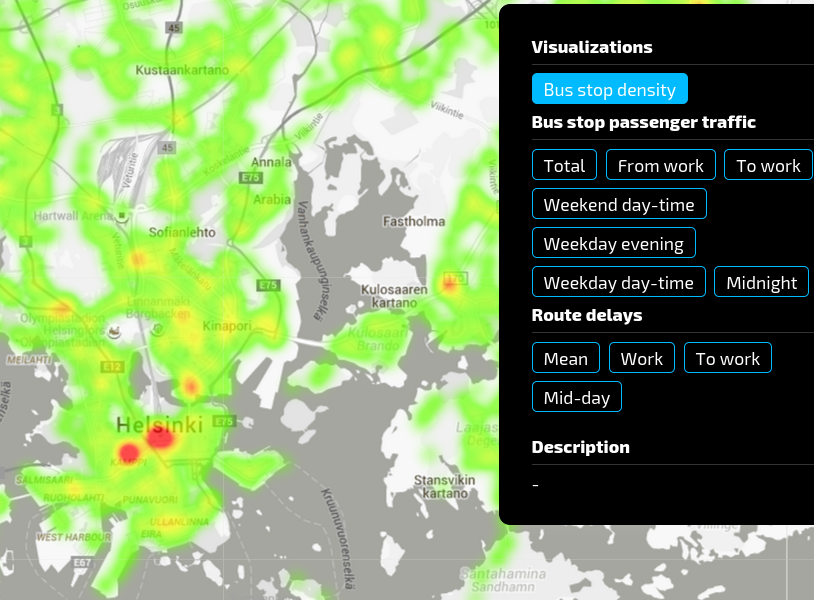
\includegraphics[width=0.47\textwidth]{stop_density.png}}
\subfigure[Average route delay.]{\label{fig:modes2}
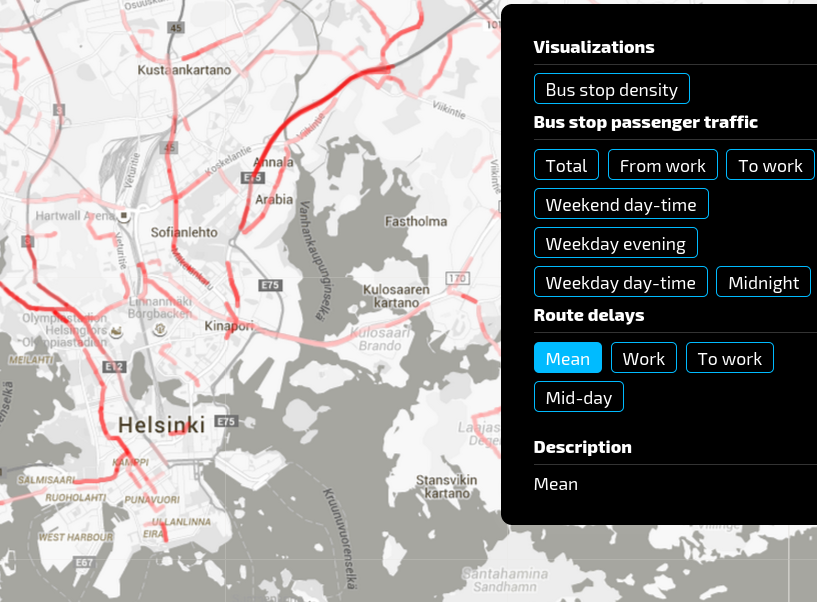
\includegraphics[width=0.47\textwidth]{route_delays.png}}
\caption{Two visualization modes illustrated. \textbf{(a)} Bus stop density. 
\textbf{(b)} Average delay at the end of the route when comparing the actual 
and the scheduled passing time.}
\label{fig:modes}
\end{figure}

A Git repository for the project can be found at:
\begin{itemize}
\item[] \url{https://github.com/asolin/aalto-data-science-hackathon}
\end{itemize}
which contains the front-end code under the \texttt{site} directory.

\subsection{Back-end}

We have stored the HSL dataset into an SQLite database in order to be 
able to compute the required quantities efficiently. Summary statistics, such 
as the cumulative time spent per bus stop, can be computed by executing simple 
SQL queries. However, one such query for the whole dataset takes about 10 
minutes to complete.

The back-end is implemented in Python, and the database is accessed from the 
code using the SQLAlchemy package. The code is available in file 
\mbox{\texttt{bus\_queries.py}} under \texttt{src} directory.

The website is static and it reads precomputed quantity data from a file in 
JSON format. It should be relatively easy to make the website dynamic using 
some Python web framework, like Flask, but due to the relatively long querying 
times, we implemented a simple static website as it would not have been 
real-time in any case. If one wanted to make a dynamic website which loads the 
data without too much lag, one could limit the time frame so that not each row 
of the database would need to be aggregated.

\subsection{Spatio--temporal analysis with matrix factorization}

Instead of merely analyzing spatial patterns, we also want to visualize 
spatio--temporal patterns found in the data. One solution would be to animate 
maps over time, but we chose to use matrix factorization techniques as the 
results are easy to visualize using the static visualization tools we have
already presented.

First, we build a stop time matrix whose values correspond to the cumulative 
time spent at a given stop (column) and at a given week of the hour (row). This 
gives us a $168\times 6490$ matrix. Since the values of the matrix are always
non-negative, we factorize the matrix using non-negative matrix factorization 
(NMF). This allows us to summarize the matrix by taking $k$ leading components, 
which represent distributions over different bus stops, and the strengths 
of these components at different hours. The first NMF component is visualized 
in Figure~\ref{fig:nmf1}.

\begin{figure}
\centering
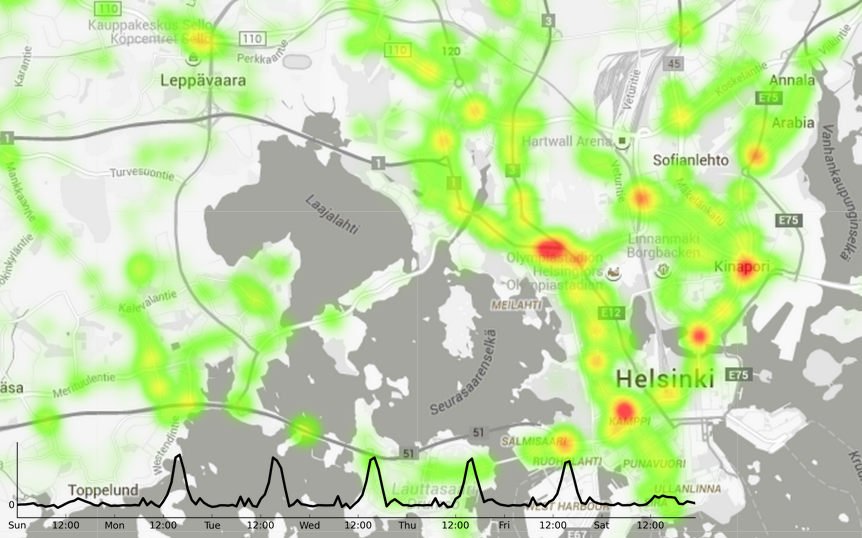
\includegraphics[width=0.8\textwidth]{nmf1.png}
\caption{The first NMF component visualized as a heatmap and its strength at 
different hours of the week. The component corresponds to the time when people 
return from work.}
\label{fig:nmf1}
\end{figure}

Similarly, we compute a route delay matrix which contains the average delay at 
the end of a route between two bus stops. The delays can also be negative if 
the bus is ahead of its schedule. Therefore, we conduct the matrix 
factorization using the principal component analysis (PCA).

The matrix factorization related code is available in file \texttt{pca.py} under
\texttt{src} directory.

\section{Results} \label{sec:res}

\subsection{Spatio--temporal analyses}

By visualizing the stop times, we were able to approximate relative passenger 
volumes stepping in or stepping out of the bus at different parts of the 
Helsinki region. The results were not too surprising; large terminal points, 
such as the city centre, Leppävaara station, and Herttoniemi metro station, 
have large volumes, probably partly because of the multitude of nearby stops 
located in these areas.

The first NMF components were also easy to interpret; 
they correspond to the traffic from/to work on weekdays, weekend traffic,
midnight traffic, etc. The midnight traffic is heavily concentrated to the city 
centre, whereas the other components spread more evenly.

The analysis of route delays also revealed clear weekly patterns. The first 
principal component corresponds to the morning and afternoon hours when people 
travel to/from work. The largest delays were exhibited in Paciuksenkatu and 
route E75 when going from the centre towards Viikki. The fact that the largest 
delays occur at peak hours in the morning and afternoon suggests that 
even though the bus time schedules try to take into account traffic volumes, 
the peak hours are not adequately accounted for.

All of these components are shown in the online demo.

\subsection{Bus waiting time}

The results of the visual analysis are probably most interesting to HSL and 
urban planners, but we also wanted to provide something for a regular 
passenger. One relevant question for the people who have troubles leaving for 
the bus stop on time is the following: \emph{What is the probability that I 
have already missed the bus?}, when the person arrives to bus stop $x$ minutes 
before/after the scheduled departure.

To address this question, we computed the cumulative bus missing probability 
given $x$, and averaged it over all bus stops. The resulting plot is shown in 
Figure~\ref{fig:miss_prob}. The plot shows that if you arrive to the stop 
exactly when the bus is scheduled to leave, in 26~\% of the cases, the bus has 
already passed the stop, whereas by arriving one minute before, the bus 
missing probability is only 10~\%.

\begin{figure}
\centering
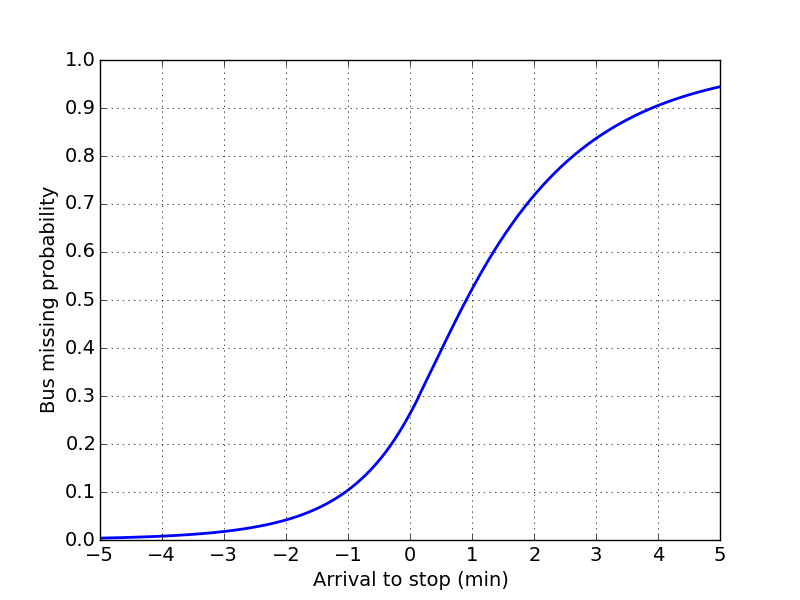
\includegraphics[width=0.7\textwidth]{bus_missing_prob.png}
\caption{Bus missing probability curve.}
\label{fig:miss_prob}
\end{figure}


\section{Conclusions and Discussion} \label{sec:conc}

We have introduced a Visual Bus Data Exploration Tool (ViBE), which can be used 
to visualize and discover spatio--temporal patterns in the bus traffic data 
released by HSL. Several intuitive patterns, e.g., corresponding to people 
going to work, were discovered from the data. The results suggest that even 
though the peak hours are accounted for in the bus time schedules, the buses 
are still delayed at these hours.

ViBE comes with at least two limitations which the user should be aware of and 
which we did not have time to fix during the hackathon. First, the heatmap 
visualization is not suitable for all types of bus stop specific data since it 
``sums'' the values of nearby stops. When computing cumulative stop time in 
order to estimate passenger volumes, as we have done in the online demo, the 
summation is justifiable, but in some other cases, if the user wanted to, e.g., 
analyze delays per stop, the summation would not be meaningful, since the 
highest delays would be shown in areas with high bus stop concentrations. 

The second limitation is that when we visualize route delays, it is not 
guaranteed that the delay has occurred exactly between the two stops 
where the colorbar is shown, since the delay is cumulative and it could have 
occurred already in the beginning of the bus line. To fix this, we should have 
computed the delay at bus stop $i+1$ and subtracted the delay at bus stop $i$. 
However, this was not trivial to compute efficiently with our database schema.

In future, ViBE could be used for analyzing individual days. It would be 
interesting to see, what kind of cascade effects are caused by special events, 
such as accidents or events attracting large crowds which can cause significant 
delay spikes at a certain part of the traffic network.

%\bibliography{sources}

\end{document}
